% 3700 words
\section*{}

In this chapter, we will first describe the methodology used to preprocess data from various sources to engineer the features for the predictive model, as informed by past literature. Second, we will outline the training model selection and evaluation process. Finally, we will discuss the methodology used to interpret the model predictions using SHAP techniques to answer the research questions. For ease of reference, the data preprocessing and feature engineering pipeline is summarised in Figure \ref{fig:preprocessing}, and an overview of the model training and prediction interpretation methodology can be found in Figure \ref{fig:methodology}. More detailed information on the data sources and the feature engineering process can be found in the Data Sources section of the Appendix.

\begin{figure}[!ht]
    \centering
    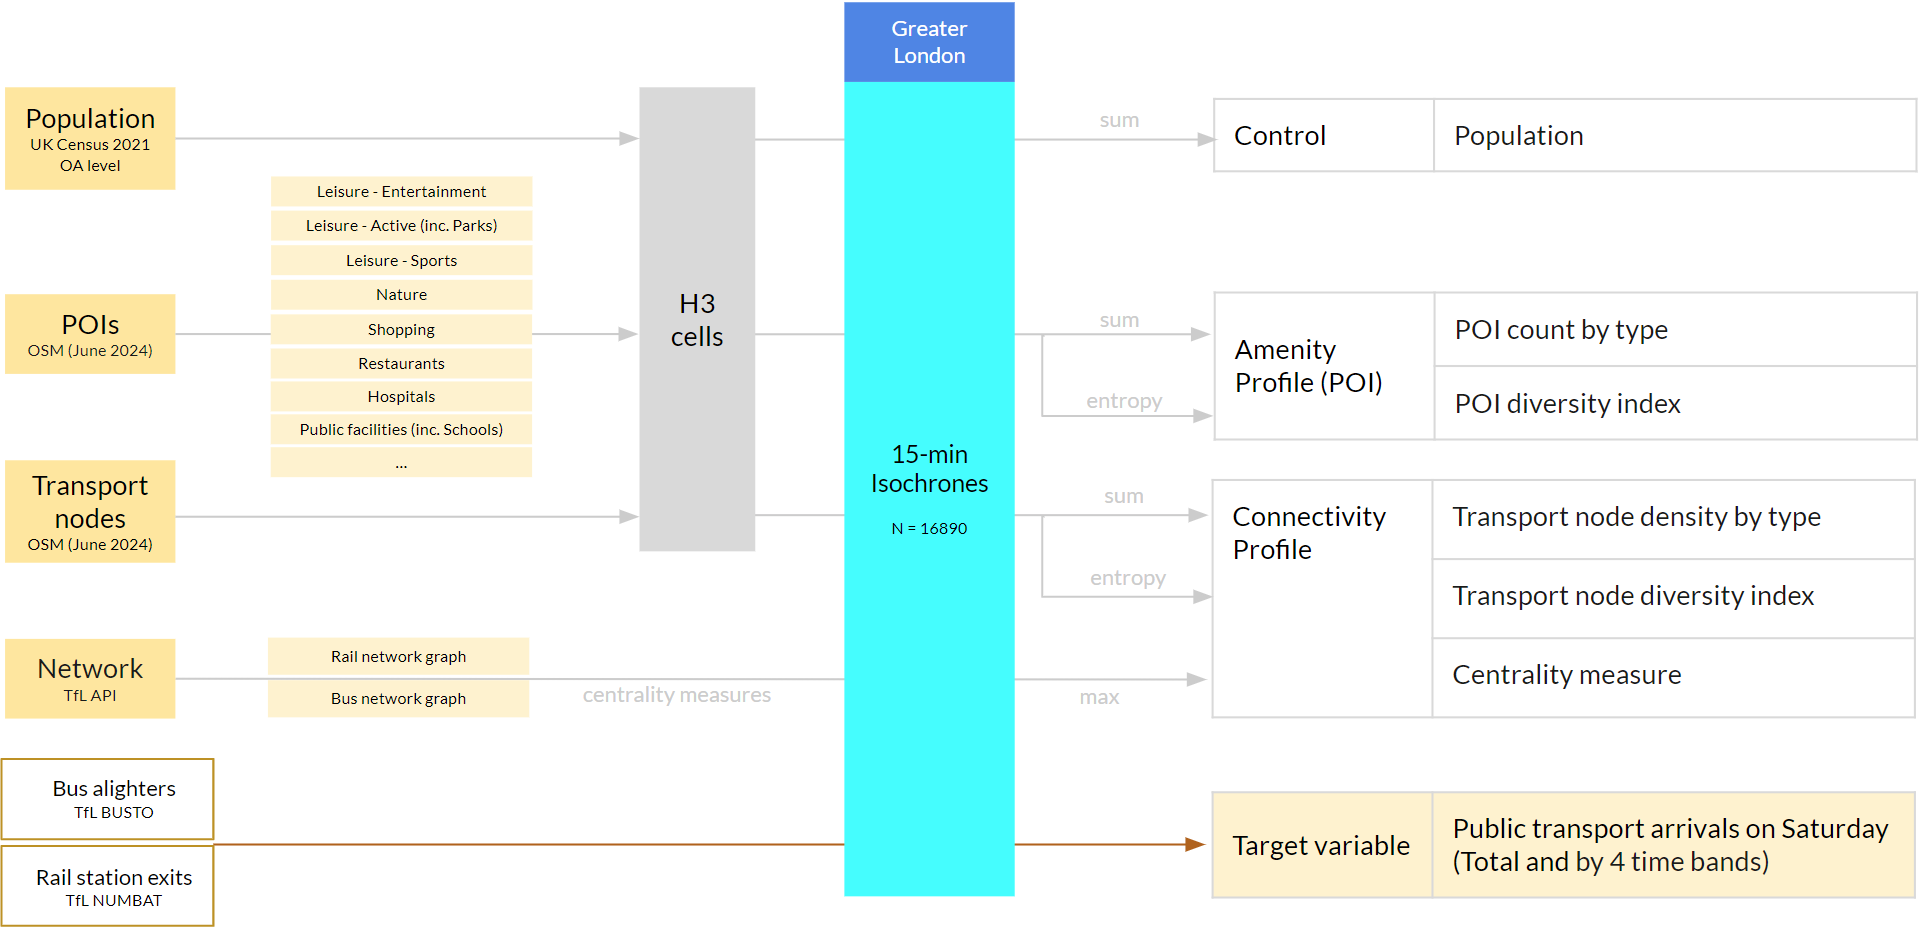
\includegraphics[width=\textwidth]{preprocessing.png}
    \caption{Overview of the feature engineering pipeline}
    \label{fig:preprocessing}
\end{figure}

\begin{figure}[!ht]
    \centering
    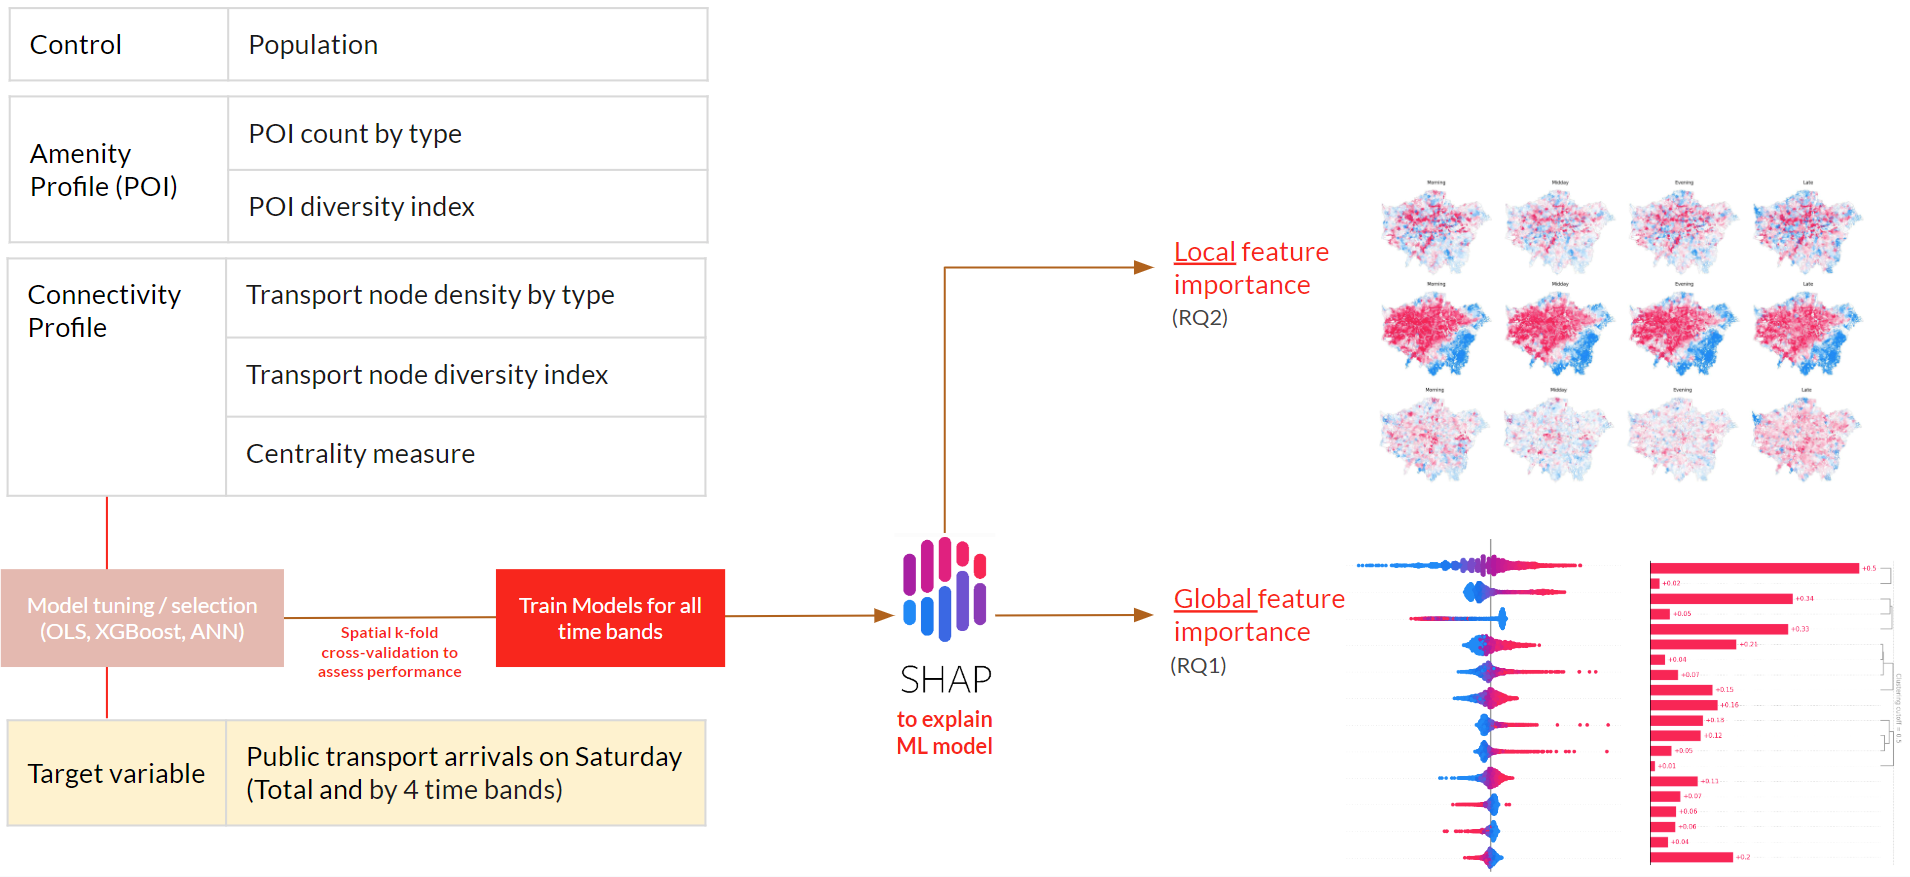
\includegraphics[width=\textwidth]{methodology.png}
    \caption{Overview of model training and SHAP explanations}
    \label{fig:methodology}
\end{figure}

\pagebreak % Force a page break
\section{Defining the spatial unit of analysis}

As features will be extracted and engineered from different data sources, the spatial unit of analysis---at which features are aggregated and the model is trained---is a crucial consideration. We will use 15-minute walking isochrones---i.e., the area that can be reached within a 15-minute walk from a point. They were generated based on initial seeds of 16,890 points distributed evenly across the Greater London region, using OpenStreetMap Pedestrian Network API (osmnx). The choice of using 15-minutes-walk isochrones as the spatial unit of analysis for our model is motivated by the following reasons: 

\begin{itemize}
    \setlength\itemsep{0em}
    \item The spatial unit should reflect how individuals interact with transport nodes and amenity POIs that are pedestrian-accessible. In contrast, Euclidean distance proximity overlooks natural barriers, such as rivers or private estates. 
    \item Human mobility in cities is not bound by administrative boundaries such as Output Areas or boroughs, and the use of overlapping isochrones allows us to capture the spatial heterogeneity of the input features and the target variables with high granularity.
    \item The 15-minute-walk specification of the isochrones aims to be aligned with the 15-minute city concept that characterises a desirable intra-neighbourhood mobility threshold. It serves as a standardised catchment area for the amenities and transport nodes that are likely to attract visitors to come and navigate on foot and, therefore, can also enable footfall estimation for local businesses within. 
    \item Lastly, the density of the spatial units is a compromise between the granularity and the computational resources required to process the data. The initial seeds of 16,890 points are centroids of H3 cells at resolution 9 needed to cover the Greater London area. 
\end{itemize}

The detailed methodology to generate the isochrones is illustrated in Figure \ref{fig:isochrones}, and two example isochrones in Central London can be seen in Figure \ref{fig:isozoom}, showing how these spatial units may vary in shapes and sizes. The following section will describe the data transformation and feature engineering process in more detail. Note that the terms spatial units of analysis or isochrones may be used interchangeably from this point in our discussion.

\begin{figure}[ht]
    \centering
    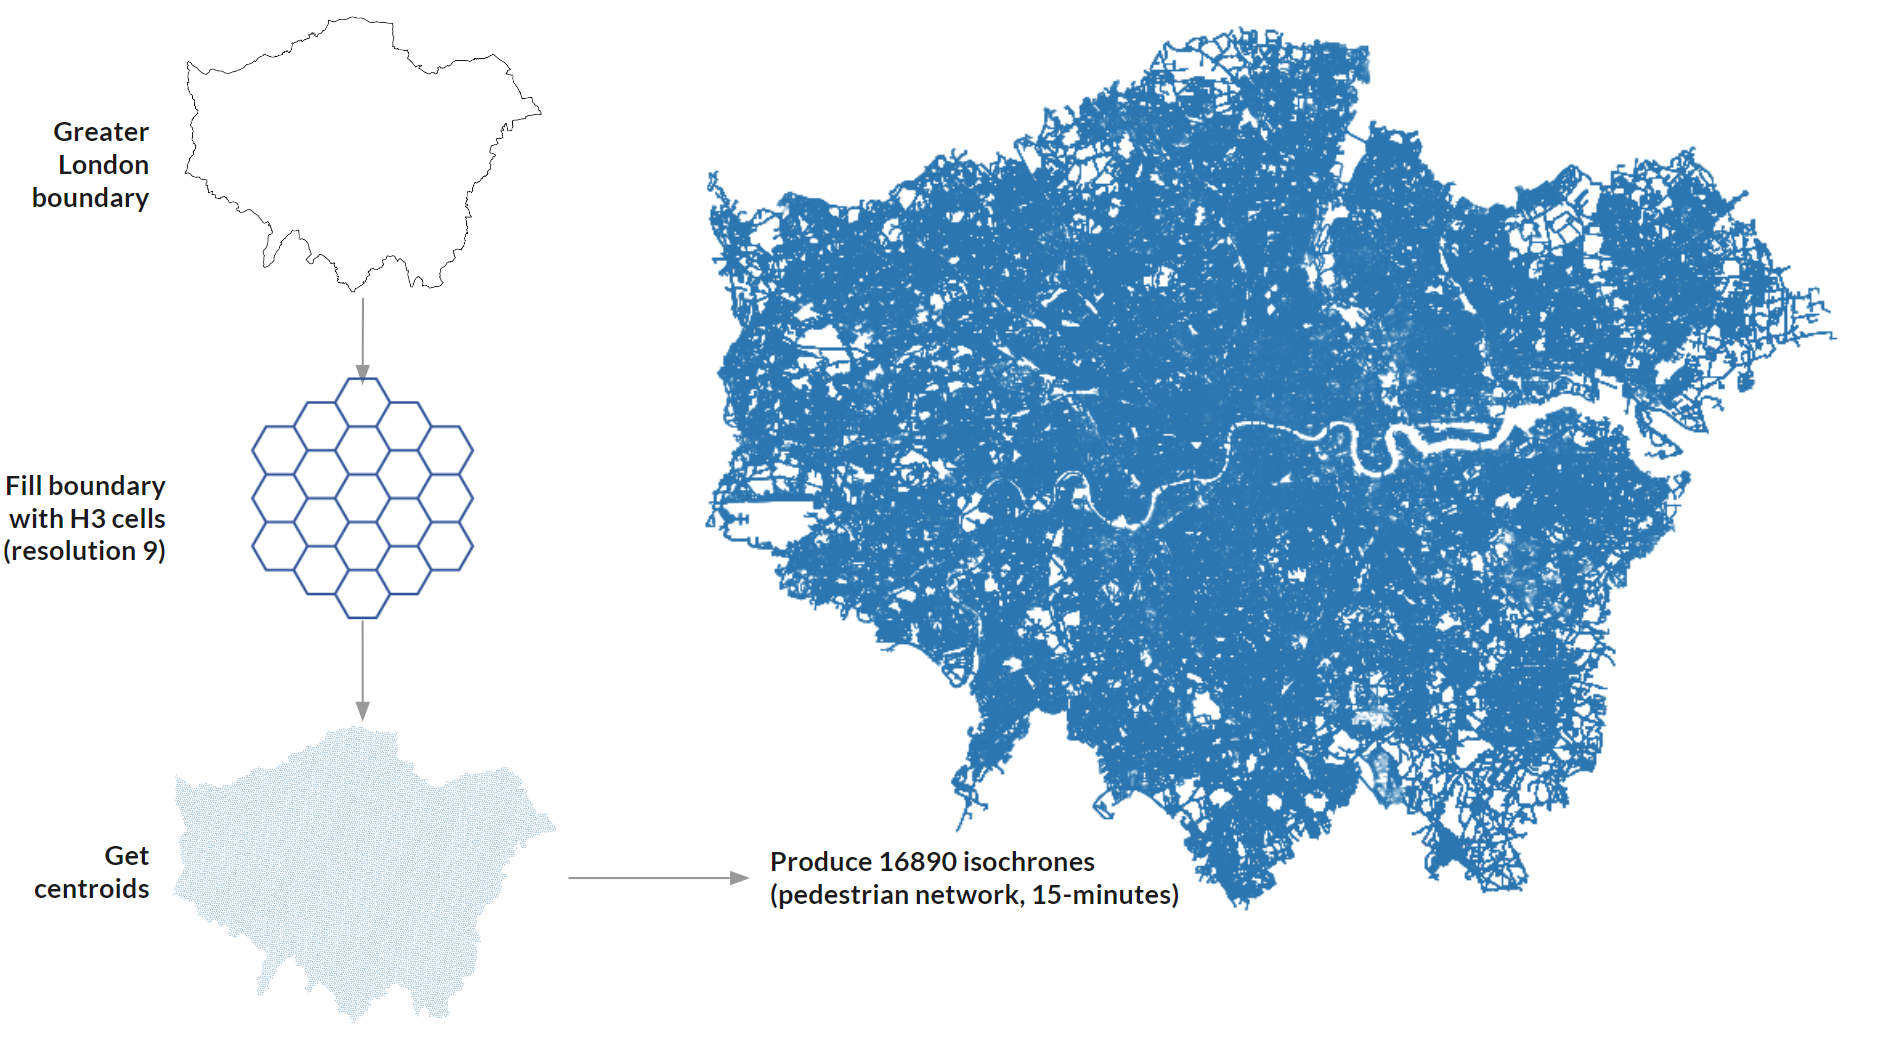
\includegraphics[width=0.8\textwidth]{isochrones.png}
    \captionsetup{justification=centering}
    \caption{Methodology to generate 16,890 isochrones as the spatial unit of analysis}
    \label{fig:isochrones}
\end{figure}

\begin{figure}[!ht]
    \centering
    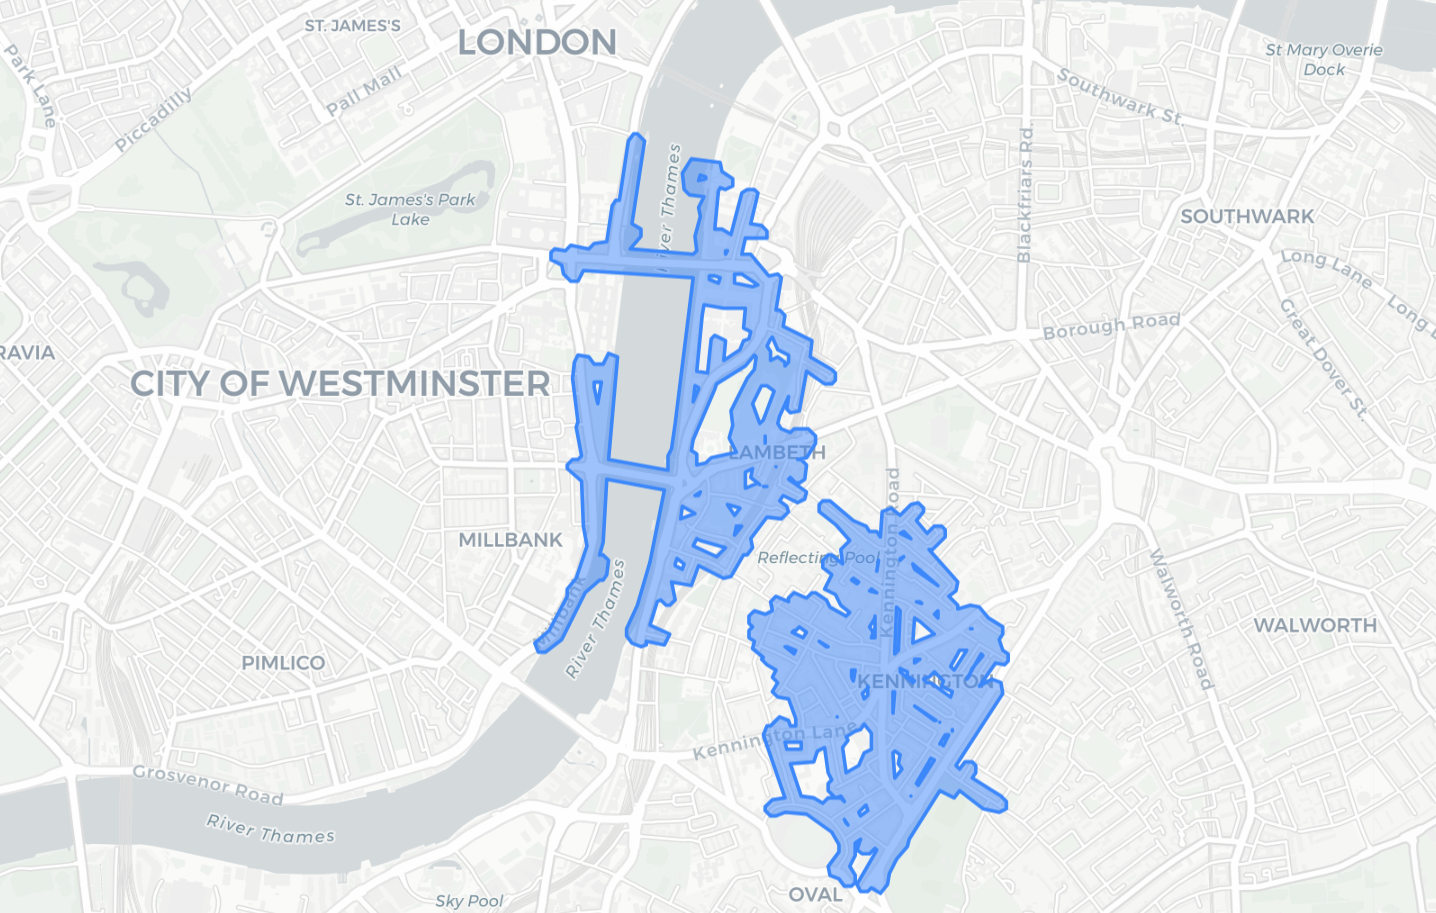
\includegraphics[width=0.7\textwidth]{isozoom.png}
    \caption{Two example isochrones as spatial units of analysis located in Central London}
    \label{fig:isozoom}
\end{figure}


\pagebreak[4] % Force a page break
\section{Data Preprocessing}
\subsection{Aggregating target variables}

\textbf{Total arrivals}, i.e., the average number of passengers who exit a station or alight from a bus\footnote{The station exit and bus alighting data are provided as open data by Transport for London based on smartcard tap data and other inference methods. See Open Data Sources in the Appendix for further clarification.} within a spatial unit on a Saturday, are the target variables for our model as a proxy for trip attractiveness. The aggregation results are illustrated in Figure \ref{fig:ptarrival}, which shows the total figures and the figures aggregated into the four time bands. The Total figures show an apparent concentration of passenger arrivals in Central London, with the highest number of passengers arriving at transport nodes. In contrast, the time band figures show a similar pattern, with the highest number of passengers arriving during the Midday and Evening time bands (10:00-19:00 and 19:00-22:00, respectively). Meanwhile, the Morning and Late time bands show lower numbers of passengers using the system due to early hours in the day on weekends and sparser night services, respectively. Lastly, since the target variable has a highly right-skewed distribution, we opt for a log transformation (shown in Figure \ref{fig:rawlog}) to the target variable to normalise the distribution and improve the model's performance, which will be corroborated in the Results section.

\begin{figure}[!ht]
    \centering
    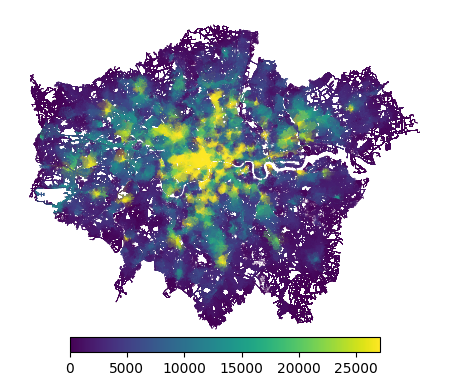
\includegraphics[width=0.5\textwidth]{pt_arrival_total.png}
    \centering
    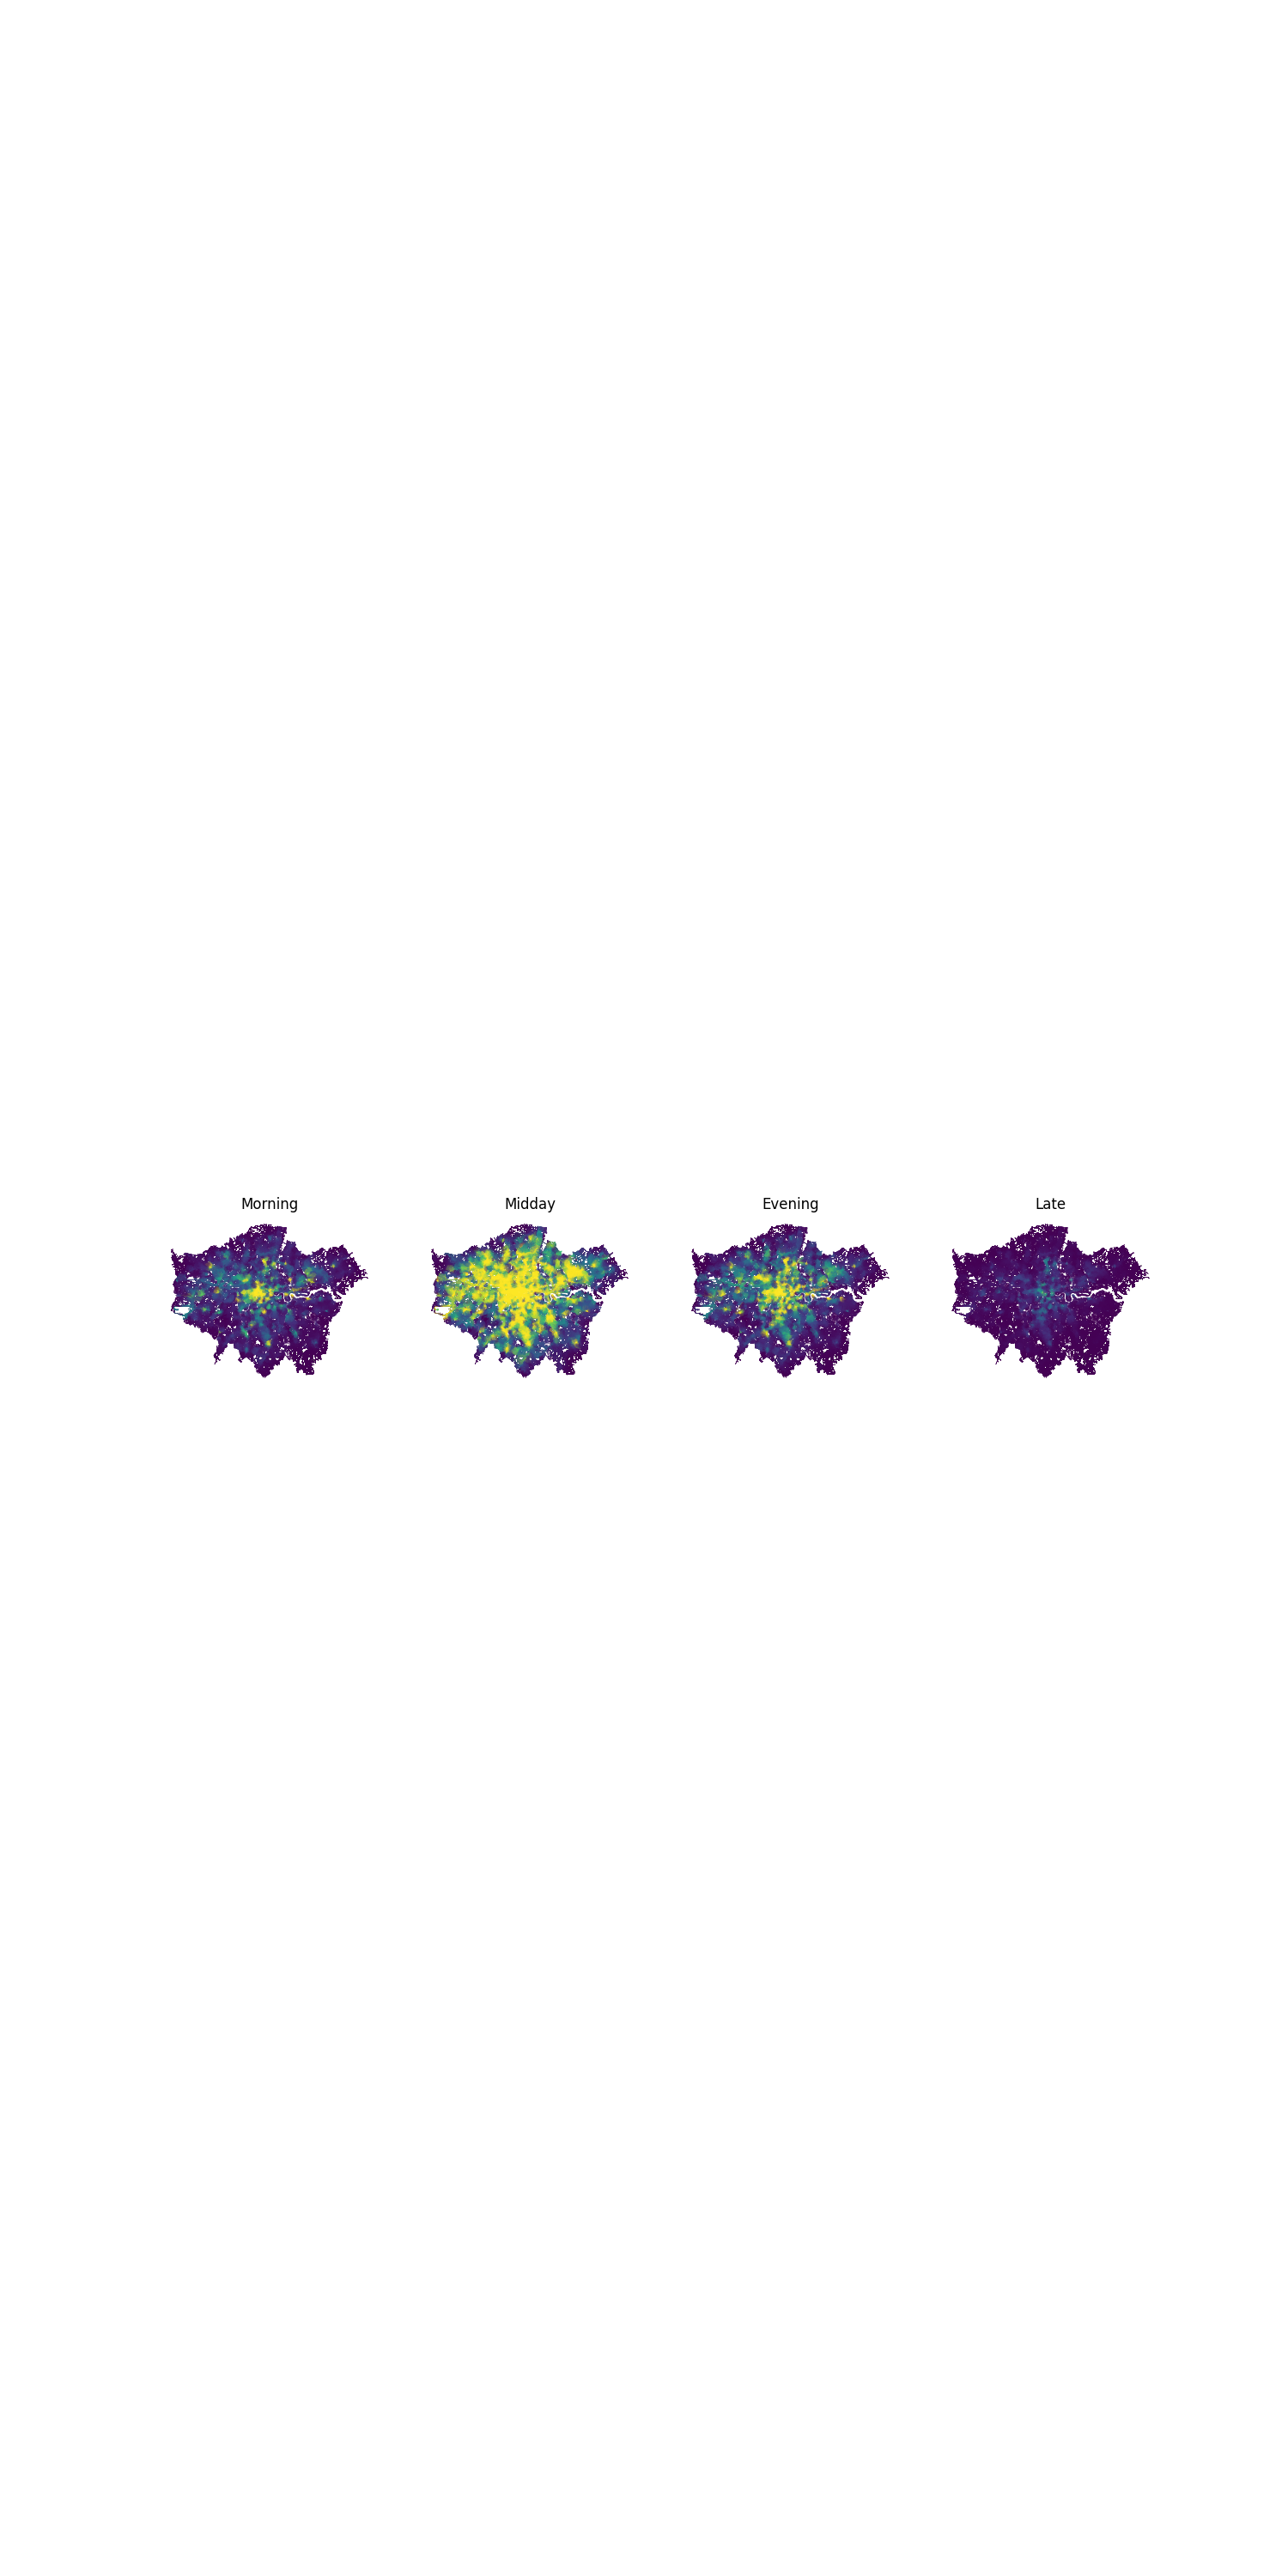
\includegraphics[width=0.75\textwidth]{pt_arrival_timeband.png}
    \captionsetup{justification=centering}
    \caption{Public transport arrivals on an average Saturday, spatially aggregated to the spatial units. \textit{Top} Total, \textit{Bottom} By time band.}
    \label{fig:ptarrival}
\end{figure}

\begin{figure}[!hb]
    \centering
    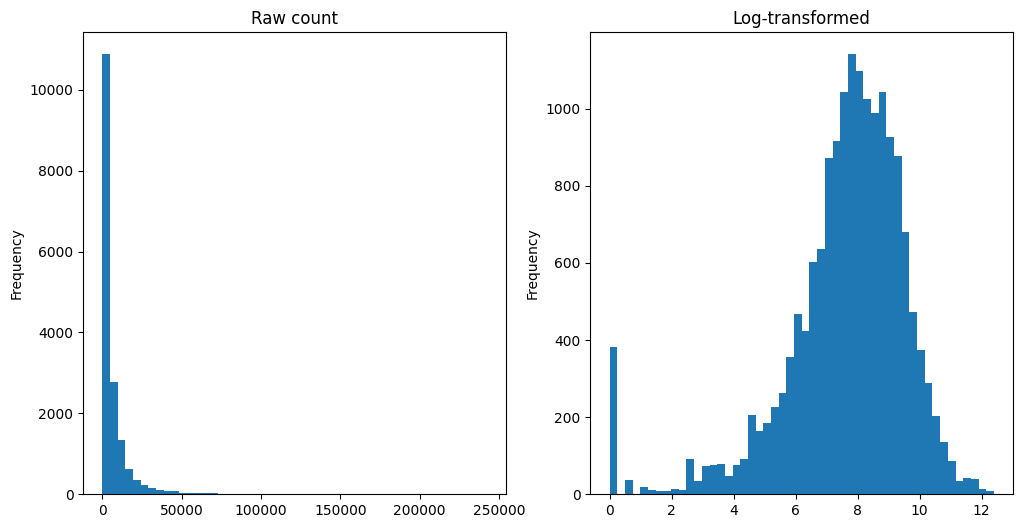
\includegraphics[width=0.5\textwidth]{raw-log.png}
    \captionsetup{justification=centering}
    \caption{Distribution of the Total arrivals as raw count (left) and log-transformed (right). (Note: Similar transformations are carried out for arrivals by each of the four time bands)}
    \label{fig:rawlog}
\end{figure}

\subsection{Feature engineering}

\subsubsection*{Density-based features}

The density of POIs is one of the first feature types of interest for our model, which represents the intensity of amenities or transport nodes of each type in an area that we hypothesise would attract visitors as destinations. Based on \citet{cerveroTravelDemand3Ds1997}'s work, we expect a positive correlation between the density of POIs of all types and the total arrivals since an area with a high concentration of retail is expected to be more attractive than a similar-sized area with a low concentration of retail if the non-commute trip is for shopping purposes. Similarly, an area with a high concentration of transport facilities, such as stations and bus stops, is expected to accommodate a higher inflow volume of visitors. All density-related features are formulated by aggregating their counts for each spatial unit by type, resulting in a set of \textbf{16 features} (See Figure \ref{fig:poppoi})

\begin{figure}[!ht]
    \centering
    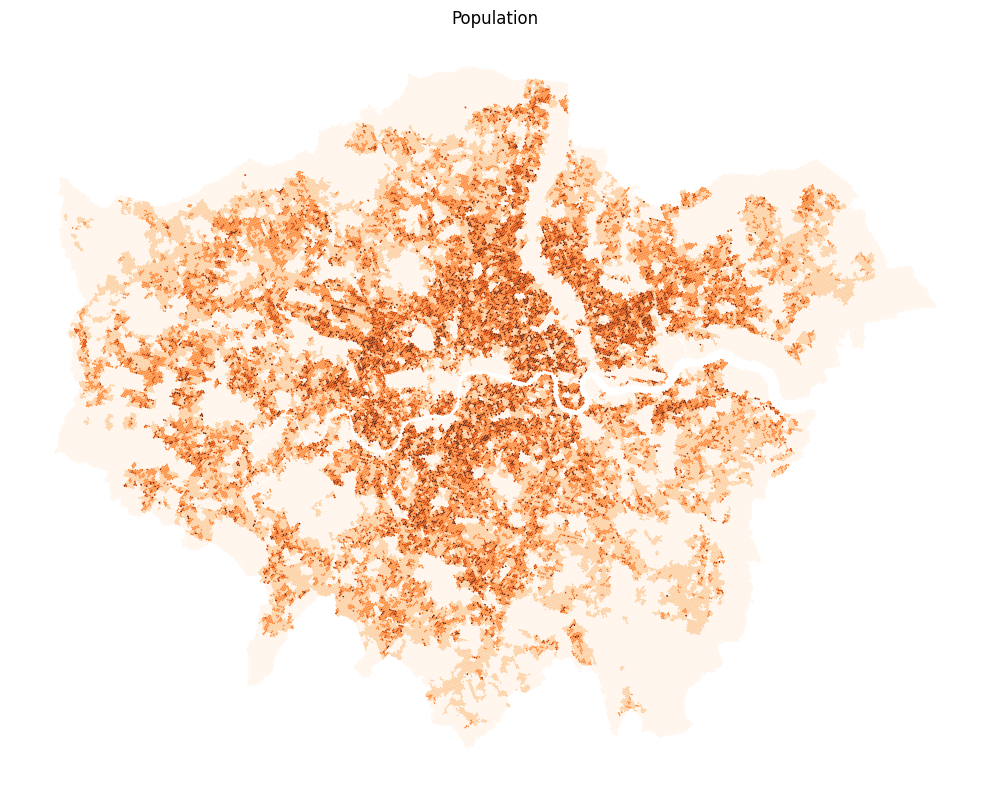
\includegraphics[width=0.4\textwidth]{POP.png}
    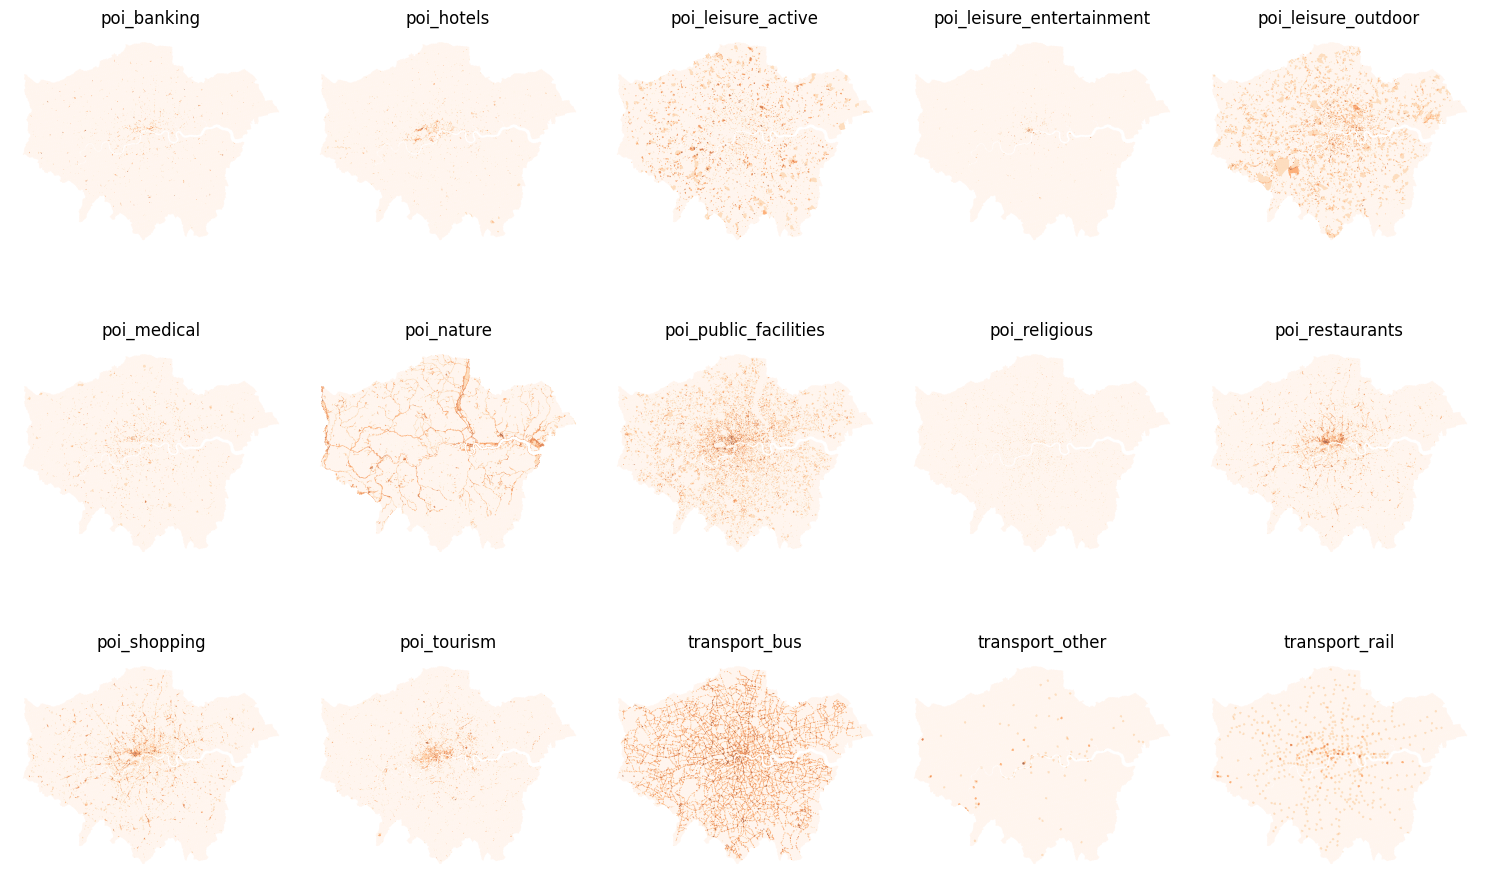
\includegraphics[width=0.9\textwidth]{POI.png}
    \captionsetup{justification=centering}
    \caption{Population, Amenity and Transport POI density by type\\(Source: UK Census 2021, OSM)}
    \label{fig:poppoi}
\end{figure}

\pagebreak[4] % Force a page break
\subsubsection*{Diversity-based features}

Diversity of Amenity POIs according to \citet{cerveroTravelDemand3Ds1997} is also an important factor that may influence the trip attractiveness of an area for certain types of non-commute travel demand. The implication is that between two neighbourhoods, all else being equal, the area that is more diverse in its amenities will be more attractive as a destination on average because of its vibrancy and the possibility it provides visitors to accomplish different tasks in one trip.

What was left under-explored by literature is the diversity of public transport facilities present in a spatial unit, which may be an important trip attractor as it is a better proxy for transit accessibility than transport node density alone. Moreover, transport diversity can also capture the modal interchange behaviour of passengers whereby they alight in a specific area to switch between different means in order to reach their final destination elsewhere. As a hypothetical example, between two areas with a similar amenity density and diversity profile, the area that can be reached with multiple transit modes and routes should be more attractive to visitors, either because it makes that area more easily accessible or because it provides opportunities for passengers to switch between different modes of transport. The latter is of critical importance. Since there is no origin-destination matrix available for the study area, its inclusion potentially helps the model disentangle the impact of modal interchange behaviour on the total arrivals, as opposed to the trip attraction factor of the area itself as a destination.

\citet{cerveroTravelDemand3Ds1997} conceptualised diversity in the form of \textit{entropy}. Entropy, a concept that originated in information theory, is the average amount of information conveyed by an event when considering all possible outcomes. \citet{battyEntropyComplexitySpatial2014} further adapted it to convey complexity in a spatial system. Interestingly, they also considered the increase of spatial entropy to be a trade-off between the density of amenity types and the unique types of amenity present, which stands in competition with other density-based features created. Therefore, including entropy as a measure of POI diversity could help us visualise this trade-off as the model is trained. We intend to replicate the approach used by both of the cited works above and adopt the formulation of entropy introduced by \citet{shannonMathematicalTheoryCommunication1948} to calculate the diversity index of amenity POIs in each spatial unit as follows:

\begin{equation}
    H = -\sum_{i=1}^{n} p_i \ln p_i
\end{equation}

\noindent where $p_i$ is the proportion of the $i$-th POI class in the total number of POIs in the spatial unit, and $n$ is the total number of POI classes being considered. The entropy index ranges from 0 to $\ln n$, where 0 indicates no diversity and $\ln n$ indicates maximum diversity, which is then normalised to the 0-1 range. Based on this definition, we will engineer \textbf{3 features} related to the diversity of amenity POIs and transport POIs, further explained as follows:

\begin{itemize}
    \setlength\itemsep{0em}
    \item \textit{Amenity POI}: 12 amenity POI classes are considered for the calculation of the diversity index for each spatial unit (see Table \ref{tab:osmpoi}). Looking at the 10\% highest values of the diversity index in Figure \ref{fig:diversity}, we can see that the most diverse areas are located throughout the Greater London area, which urban studies literature links to activity centres or neighbourhoods. As a whole, the distribution of the diversity index is right-skewed, indicating a pluricentric urban structure in Greater London.
    \item \textit{Transport POI diversity by mode}: 3 transport POI classes (bus stops, rail stations, other hubs) are considered for the calculation of the diversity index for each spatial unit (see Table \ref{tab:osmpoi}). The top 10\% values of the diversity index are mapped in Figure \ref{fig:diversity}, showing that the most diverse areas are located around important transport intermodal hubs, such as national rail stations, airports, and ferry piers.
    \item \textit{Transport POI diversity by route option}: A more granular transport diversity index is calculated for the transport POIs, considering the different bus routes and train services the transport POIs in each spatial unit serve. The top 10\% values of the diversity index are mapped in Figure \ref{fig:diversity}, showing that the most transport-option diverse areas are not only intermodal hubs but also areas around arteries where many bus routes or rail services converge.
\end{itemize}

\begin{figure}[ht]
    \centering
    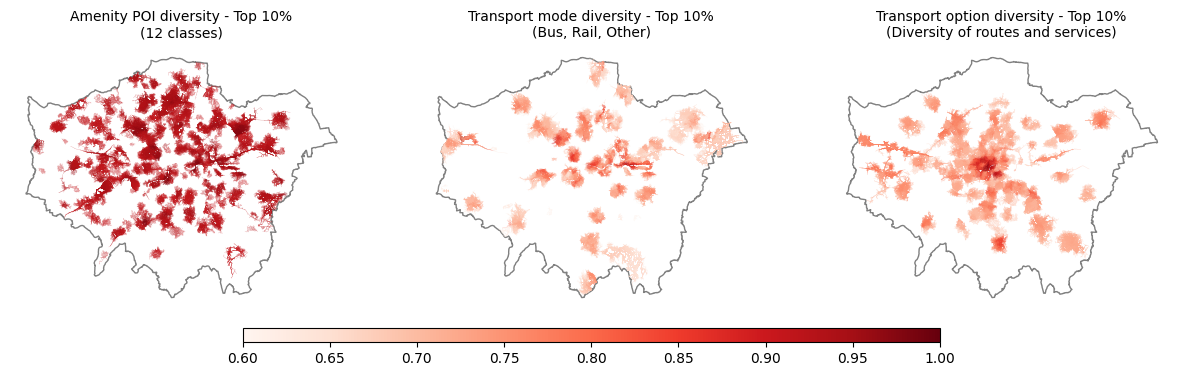
\includegraphics[width=\textwidth]{divmap.png}
    \centering
    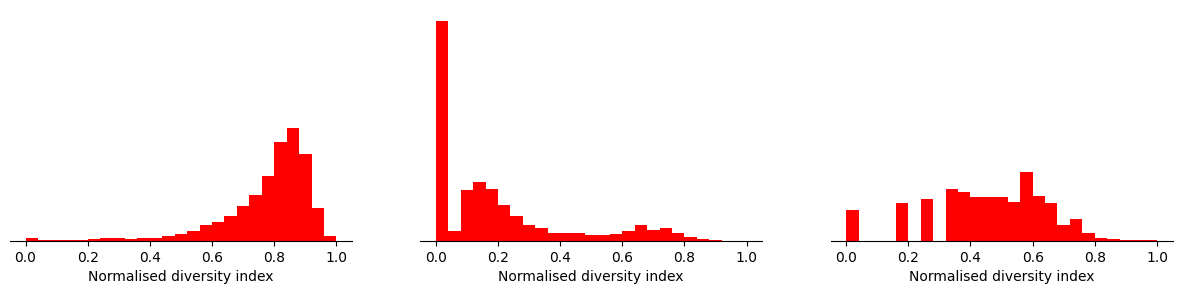
\includegraphics[width=\textwidth]{divhisto.png}
    \captionsetup{justification=centering}
    \caption{Normalised diversity indices for Amenity POIs, Transport POIs by mode and by route options. \textit{Top}: Mapping top 10\% values, \textit{Bottom}: Distribution of diversity indices}
    \label{fig:diversity}
\end{figure}

\begin{figure}[!hbt]
    \centering
    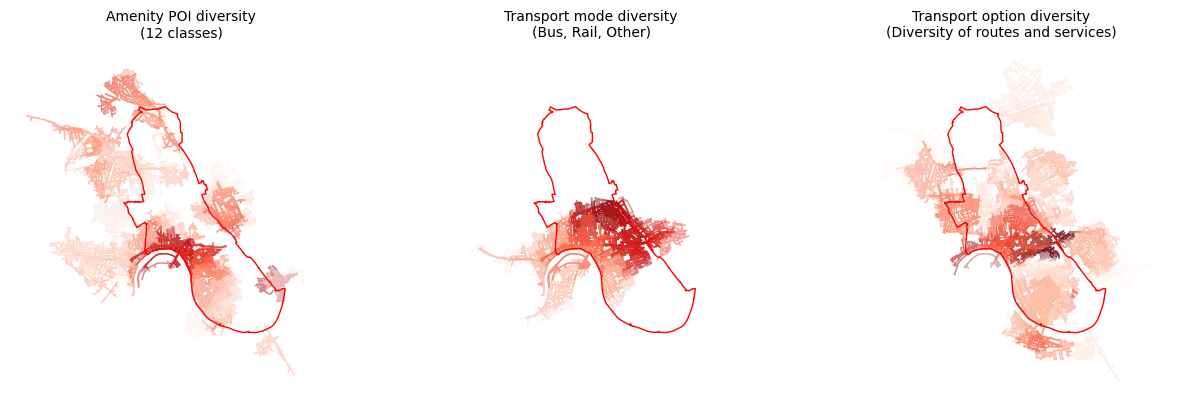
\includegraphics[width=\textwidth]{divboro.png}
    \captionsetup{justification=centering}
    \caption{Top 10\% values of 3 diversity indices\\Borough: Hammersmith-and-Fulham}
    \label{fig:diversityboro}
\end{figure}

The inclusion of both transport diversity indices aims to provide complementary information to the model, as they capture different factors to explain why an area receives more or less arriving passengers. High transport mode diversity indicates a high possibility that the area facilitates modal interchange for onward travel (such as long-distance intercity or cross-city trips), whereas high transport route diversity, in addition to that, indicates a high possibility that the area is locally well-connected with reasonable frequency. Zooming into a specific area, such as the Hammersmith and Fulham borough, we can see a slight divergence between the two transport diversity indices (Figure \ref{fig:diversityboro}). The Shepherd's Bus area has a higher transport mode diversity index thanks to the existence of national rail services (Southern Railways) beyond Tube and buses. In contrast, the area around Earl's Court has a higher transport option diversity index due to the presence of multiple local bus routes converging in the area.

\pagebreak[4] % Force a page break
\subsubsection*{Centrality-based features}

Whereas the public transport diversity index, previously discussed, captures the variety of transport options available in an area, it obscures one aspect of accessibility in relation to other areas in London using the public transport network. Centrality-based features add yet another layer of information to the model, capturing the importance of a bus stop or a station in relation to the whole network. For example, between two hypothetical areas with similar diversity of transport options (e.g., both are served by five bus routes), the area with a higher centrality measure may be more attractive to visitors because it is more 'accessible' from other areas on average. 

\begin{figure}[hbt]
    \centering
    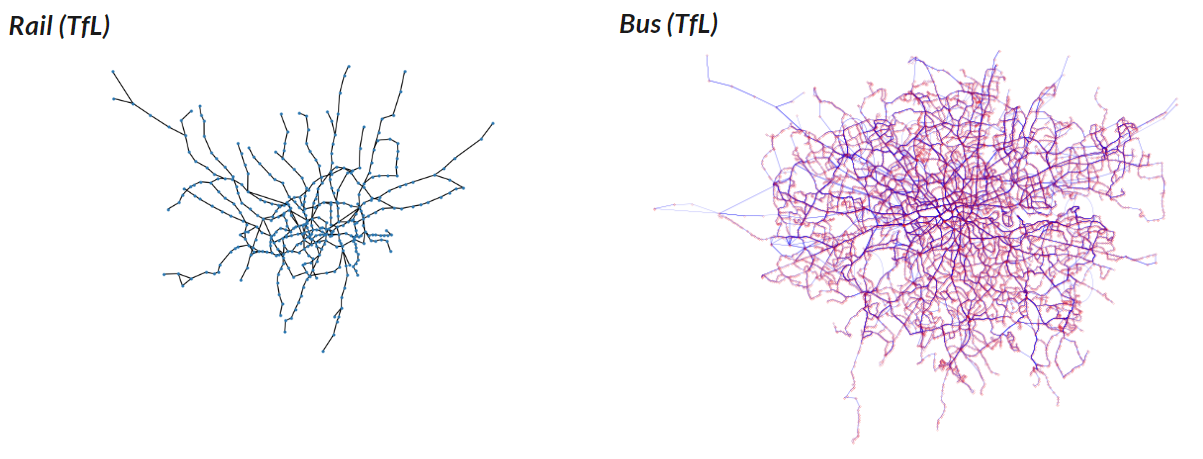
\includegraphics[width=0.8\textwidth]{network.png}
    \captionsetup{justification=centering}
    \caption{Network graphs of TfL Bus (left) and Rail (right) networks\\Constructed based on TfL API data}
    \label{fig:network}
\end{figure}

\begin{figure}[!ht]
    \centering
    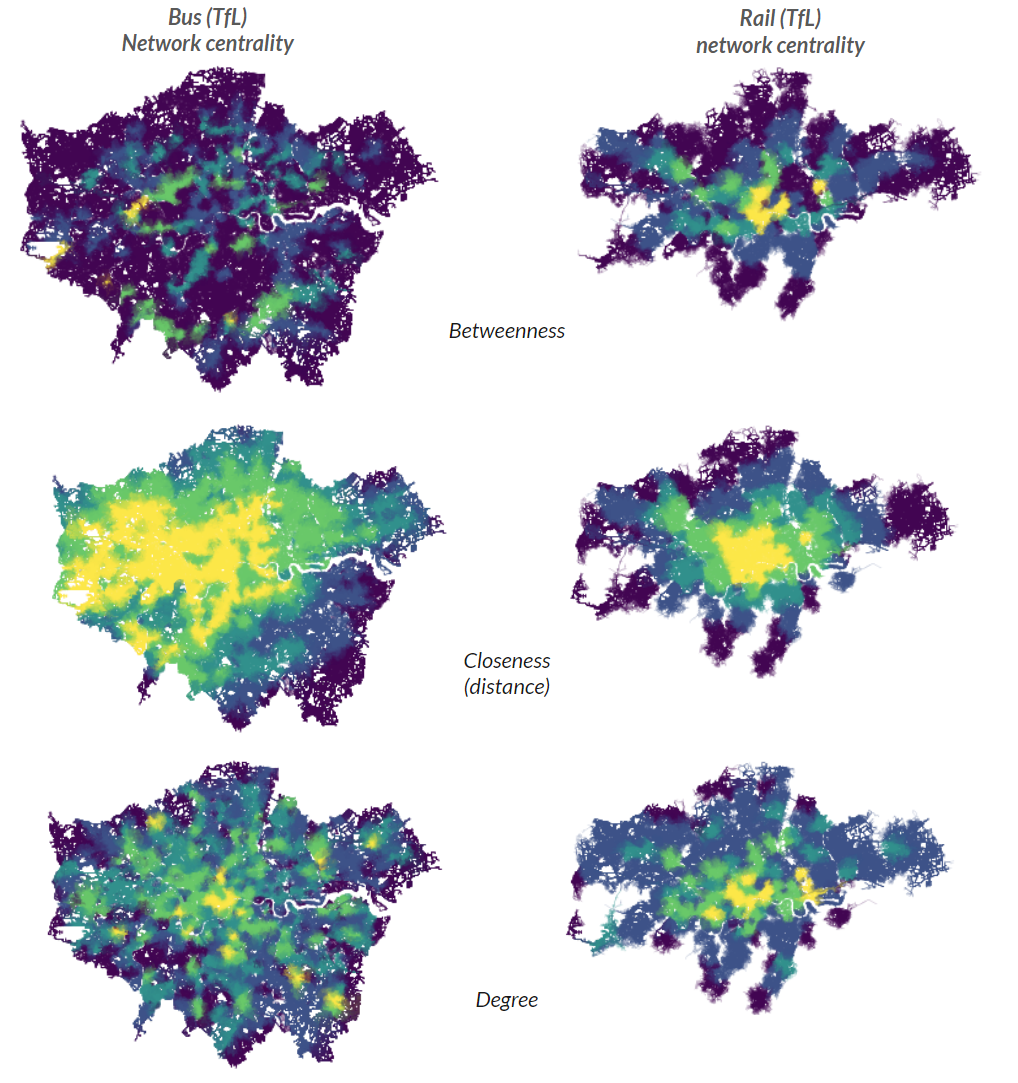
\includegraphics[width=0.8\textwidth]{centrality.png}
    \captionsetup{justification=centering}
    \caption{Mapping three centrality measures of spatial units\\on the Rail (left) and Bus (right) networks}
    \label{fig:centrality}
\end{figure}

First, we construct the network graph of the TfL Bus and the TfL Tube and Rail networks from open data (See Figure \ref{fig:network}), with nodes representing the stops or stations and the edges representing routes or lines. Due to the lack of data related to travel time and scheduling, we abstain from combining the two networks into a multi-layered network, which would have allowed us to consider the whole public transport network as one connected component. Instead, we will calculate the following centrality measures for all the nodes in the Rail and Bus networks separately, resulting in a set of 6 node attributes:

\pagebreak[4] % Force a page break
\begin{itemize}
    \setlength\itemsep{0em}
    \item \textit{Degree centrality}: The number of direct connections a node has. A high degree of centrality indicates that the node is well-connected to other nodes in the network (i.e., many routes available).
    \item \textit{Closeness centrality}: The average shortest path length from a node to all other nodes in the network. A high closeness centrality indicates that the node is close to other nodes in the network (i.e., centrally located). 
    \item \textit{Betweenness centrality}: The number of shortest paths that pass through a node in the network. A high betweenness centrality indicates that the node is an important bridge between other nodes in the network (i.e., transport hubs).
\end{itemize}

Finally, to incorporate calculated attributes of the nodes into \textbf{6 features} of centrality, we will consider all the nodes in each spatial unit and extract the maximum attribute values. In other words, the centrality feature of a spatial unit has the value of the rail or bus transport node with the highest centrality measure of each of the six attributes. The mapping of the centrality measures to the spatial units is illustrated in Figure \ref{fig:centrality}.

\subsection{Incorporating spatial lags as a feature}

In summary, the feature engineering process thus far has resulted in a total of \textbf{25 features} that will be used to train the model to predict the (log-transformed) public transport arrivals in a given spatial unit. The features are summarised in Table \ref{tab:features}.

\begin{table}[!ht]
    \centering
    \renewcommand{\arraystretch}{1.25}
    \begin{tabular}{|r||l|}
        \hline
        \rowcolor{lightgray}
        \textbf{No.} & \textbf{Feature} \\
        \hline
        1 & Population density \\
        2-13 & Amenity POI density by type (12) \\
        14-16 & Transport POI density by type (3) \\
        17 & Amenity POI diversity index \\
        18 & Transport POI diversity index by mode \\
        19 & Transport POI diversity index by route option \\
        20-25 & Bus and Rail centrality measures (Degree, Closeness, Betweenness) (6) \\
        \hline
    \end{tabular}
    \caption{Summary of the 25 main features engineered for the model}
    \label{tab:features}
\end{table}

When working with machine learning models with data in a closed spatial system such as the Greater London area, it is important to consider the spatial autocorrelation in the target variable. In the context of our analysis, the number of passengers arriving in an area is likely correlated with the number of passengers arriving in nearby areas. Although deep learning models' parameters and hyperparameters can be made more complex and tuned to reach a high degree of prediction accuracy without considering the spatial aspect of the dataset, accounting for potential spatial autocorrelation could reduce the probability of biased outcomes even with a relatively low-complexity and high-interpretability architecture, e.g. tree-based models \citep{meyerImportanceSpatialPredictor2019}.

The indication of spatial autocorrelation in the target variables is confirmed by the Local Indicators of Spatial Association (LISA) analysis, which shows the presence of spatial clusters in the target variables (Figure \ref{fig:lisacluster}), using Local Moran's I indicators. If spatial information among these spatial units is provided to the model during tuning and evaluation, we could improve accuracy further, especially in these localities that make up more than 50\% of the study area.  

\begin{figure}[ht]
    \centering
    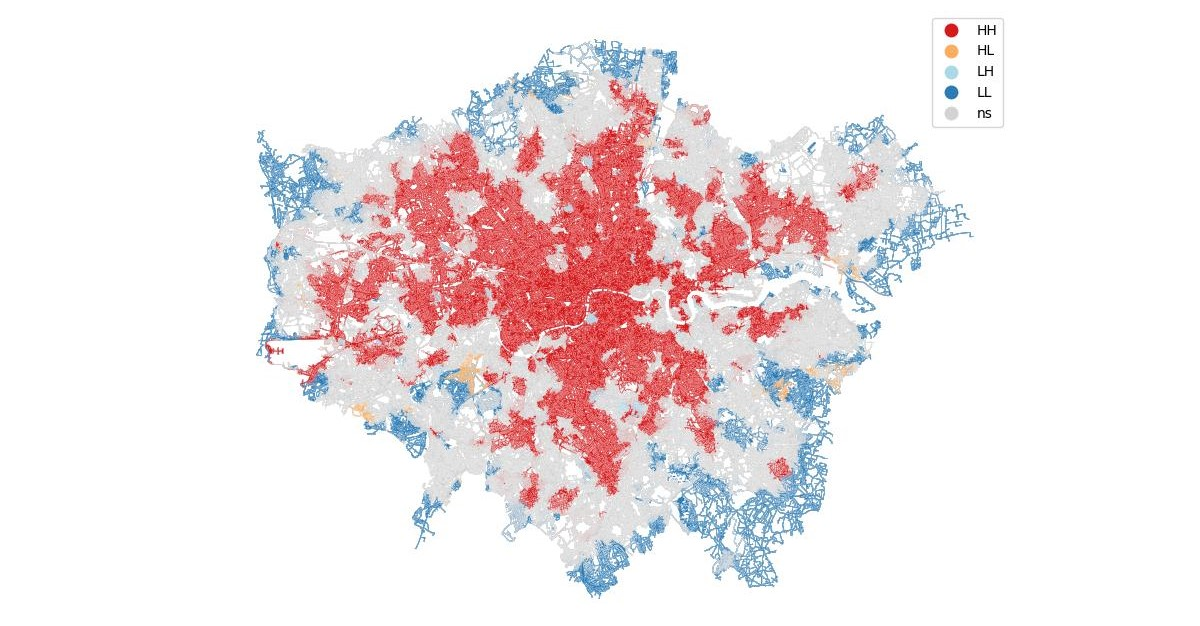
\includegraphics[width=\textwidth]{lisa_Total.jpg}
    \captionsetup{justification=centering}
    \caption{LISA cluster map of Total arrivals showing local spatial autocorrelation\\Global Moran's I: 0.742 (High spatial autocorrelation)}
    \label{fig:lisacluster}
\end{figure}

To address this issue, \citet{liuIncorporatingSpatialAutocorrelation2022} proposed incorporating spatial lag into the model as a feature. More specifically, the authors have concluded that when spatial features were induced in the random forest model, the global spatial autocorrelation among the predictions' residuals was significantly reduced, leading to higher validation accuracy. For our analysis, the spatial lag feature of each spatial unit is calculated as the average number of passengers arriving at neighbouring isochrones\footnote{The choice of the distance band of 750m was calibrated to ensure all spatial units have neighbours, i.e., there are no islands.}. The creation of a \textbf{Spatial Lag features} is replicated for the total arrival counts, as well as for each time band, resulting in a set of additional features to be included to train the model in predicting the corresponding target variable.

\begin{table}[ht]
    \centering
    \renewcommand{\arraystretch}{1.5}
    \begin{tabular}{|c r || c c l|}
        \hline
        \rowcolor{lightgray}
        \textbf{No.} & \textbf{Target variable} & \textbf{Main Features} & &\textbf{Spatial Lag Feature}\\
        
        \hline
        1 & Total arrivals  &  \multirow{5}{10em}{Population, amenity and accessibility profile (25 features)} 
                                &  \multirow{5}{*}{+}       &   Spatial Lag - Total arrivals    \\ 
        2 & Morning arrivals    &                       &   &   Spatial Lag - Morning arrivals  \\ 
        3 & Midday arrivals     &                       &   &   Spatial Lag - Midday arrivals   \\ 
        4 & Evening arrivals    &                       &   &   Spatial Lag - Evening arrivals  \\ 
        5 & Late arrivals       &                       &   &   Spatial Lag - Late arrivals     \\
        \hline
    \end{tabular}
    \caption{Mapping spatial lag features to predict corresponding target variables}
    \label{tab:spatiallag}
\end{table}


\pagebreak[4] % Force a page break
\section{Model selection and interpretation}

As previously explored through relevant literature, we are faced with an important decision when attempting to model the non-commute travel demand in the Greater London area based on variables related to the built environments, such as the amenity profile and the connectivity profile. More specifically, the choice is between using a machine learning model---which prioritises prediction accuracy and can handle heterogeneous data, and a spatial-statistical one---which prioritises interpretability and requires more stringent requirements of the explanatory variables. Although spatial statistical models such as the Spatial Lag Model or Geographically Weighted Regression are standard for such analysis, \citet{liExtractingSpatialEffects2022} has shown that machine learning models can capture spatial effects if spatial information is provided, and the appropriate Machine Learning explanation technique is used. This work aims to demonstrate the use of SHAP explanation on a fine-tuned prediction model to provide insights into the geographically varying effect of the features on the predictions. Figure \ref{fig:methodology} provides an overview of the model training and interpretation process.

\subsubsection*{Model evaluation}
Firstly, we will compare the performance of three machine learning models: \textit{Linear Regression, Gradient Boosting, and Neural Network} in predicting Total arrivals. As we are working within a spatial system with a high degree of spatial autocorrelation demonstrated earlier, special attention will be paid to spatial cross-validation in hyperparameter tuning and evaluation because random cross-validation and train-test splits are not able to prevent train-test data leakage, which inflates the accuracy score. 

More specifically, the model tuning and evaluation process will be carried out using a nested 10-fold cross-validation approach introduced by \citet{schratzPerformanceEvaluationHyperparameter2018}, with $R^2$ as the performance metric. The nested cross-validation approach is illustrated in Figure \ref{fig:spatialnested}, where the inner loop tunes the model's hyperparameters, and the outer loop is used to evaluate the model's performance. The spatial 10-fold cross-validation splits for our datasets (see Figure \ref{fig:kfold} in Appendix) ensure that the training and test sets in the inner and the outer folds are spatially distinct. The model and its hyperparameters with the highest $R^2$ score will be selected as the best model to fit the entire dataset for further analysis\footnote{Although the model tuning and selection process is only performed on Total Arrivals as the target variable for simplicity, the chosen model will be applied to predict arrivals by time bands.}.

\begin{figure}[!ht]
    \centering
    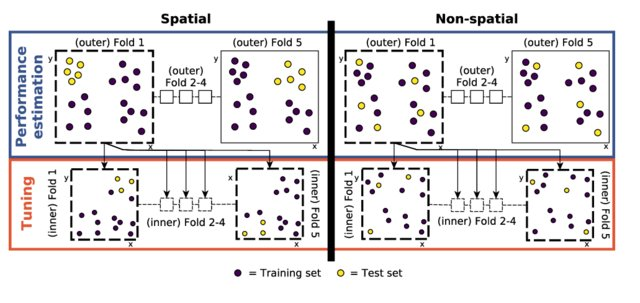
\includegraphics[width=\textwidth]{spatialvalidation.jpg}
    \captionsetup{justification=centering}
    \caption{Spatial vs. non-spatial nested cross-validation using 5-folds for hyperparameter tuning and performance evaluation. This technique helps ensure the training and test sets in both the inner and the outer folds are spatially clustered to avoid data leakage\\ Source: \citet{schratzPerformanceEvaluationHyperparameter2018}}
    \label{fig:spatialnested}
\end{figure}

\subsubsection*{Model interpretation}

Rooted in the work on game theory, SHAP tackles the challenge of fair credit allocation within a cooperative game. In this reimagined context, features in our data are the players, the set of features used for training represents the coalition, and a model prediction is the game. For each observation, the SHAP values quantify the average marginal contribution of a feature to achieve the final prediction, providing a nuanced understanding of each feature's impact on the model's predictions at the local level (i.e., for each observation)

Among other properties contributing to its popularity in Explainable AI research, it is model-agnostic and additive, meaning that the sum of all features' SHAP values equals the difference between the model's final and baseline predictions for each observation. In this scenario, given the model is spatially aware thanks to the addition of spatial lags as a feature, the outputs from this ML explanation technique share some similarities in interpretation with spatially varying coefficients of a geographically weighted regression model. Visualising features' SHAP values on a map can, therefore, provide insights into the spatial heterogeneity of the feature importance in the model's prediction, which can be used to identify hotspots of high trip attraction factors for non-commute travel demand.

While SHAP computation was initially a barrier, approaches like Kernel SHAP and Tree SHAP made available in the SHAP package have made estimation more efficient. SHAP's local interpretability and integration with popular machine learning libraries also make it a powerful tool for spatial data where feature attribution can be visualised geographically. These properties of SHAP allow us to derive our methodology to interpret the model's prediction in the context of the features engineered to answer the research questions:

\begin{itemize}
\setlength\itemsep{0em} 
    \item SHAP-based \textit{global feature importance} will be used to identify the most important features (amenity and connectivity profiles) to the model's prediction of inflow travel demand, allowing us to understand the general patterns and relationships between the features and the target variables. Since the model in question must attain a high level of accuracy before the SHAP values can be considered insightful, due care will be taken to ensure that the model is well-tuned and evaluated before proceeding with the SHAP analysis.
    \item SHAP-based \textit{local feature importance} will be used to interpret the model's prediction for individual spatial units, allowing further investigation into identifying local spatial trip attraction patterns. With spatial clustering analysis such as HDBSCAN on the local SHAP, we can also identify clusters where our main features of interest have high (or low) importance compared to others, effectively identifying hotspots of high trip attraction factors for non-commute travel demand.
\end{itemize}

The following chapter will present the results of the model training and interpretation process, followed by a discussion of the findings and their implications for the research questions and other applications.

\section{Ethical considerations}

The research exclusively utilises publicly available and anonymised data, ensuring individual privacy and confidentiality. Data sources are transparently outlined in the Appendix, and the anonymisation process mitigates re-identification risks, such as suppressing low counts in the outputs. The findings from this research may be disseminated for academic purposes to contribute to a greater understanding of urban mobility patterns, as well as with partner organisations and municipal transport authorities to inform more responsive and sustainable urban planning, transport service planning, and policy-making. The UCL Ethics Committee assessed the study's scope and methodology as minimal risk and did not require further review.